% !TEX root = manuscript.tex

\chapter{Présentation du contexte Data Science}
%\epigraph{ Nous avons divisé les données(train), en données d'entraînement et de validation.}{}
%minitoc
%\newpage
\section{Présentation des données}
\begin{flushleft}
L'ensemble de données utilisé dans ce projet provient du challenge "IST Deep Learning Workshop" sur la reconnaissance de caractères ourdou. Il se compose de trois fichiers principaux, chacun jouant un rôle spécifique dans notre pipeline d'analyse et de modélisation.
\end{flushleft}
\subsection{Structure et caractéristiques des données}
Les données sont organisées en deux ensembles principaux :

\begin{enumerate}
\item \textbf{Ensemble d'entraînement (data\_train.csv) }
\begin{itemize}
\item Nombre d'échantillons : 28 328 images de caractères ourdou
\item Structure : 786 colonnes au total
\begin{itemize}
\item \textbf{ID} : Identifiant unique de l'image
\item \textbf{Class Label} : Étiquette de classe (entier entre 0 et 39)
\item \textbf{Value 1 à Value 784} : Valeurs de pixels de l'image (784 = 28×28)
\end{itemize}
\end{itemize}
\item \textbf{Ensemble de test (data\_test\_mlp\_final.csv) :}
\begin{itemize}
\item Nombre d'échantillons : 4 880 images
\item Structure : 785 colonnes
\begin{itemize}
\item \textbf{ID}: Identifiant unique
\item \textbf{Value 1 à Value 784}: Valeurs de pixels
\item Pas de colonne d'étiquette, celle-ci devant être prédite
\end{itemize}
\end{itemize}
\item \textbf{Fichier de soumission d'exemple :}
\begin{itemize}
\item Format attendu pour la soumission des prédictions sur Kaggle
\item Structure : identifiant de l'image et classe prédite
\end{itemize}
\end{enumerate}

Aperçu des dimensions des fichiers :

\begin{figure}[h]
\centering
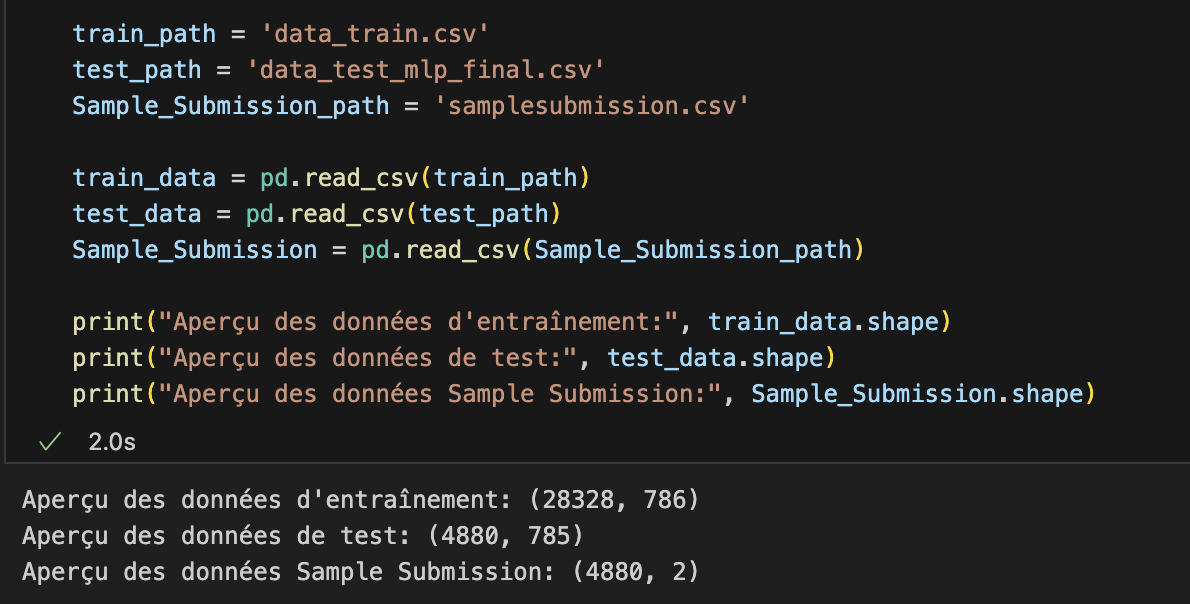
\includegraphics[width=0.7\textwidth]{figures/Aperçu.png}
\caption{Aperçu des dimensions des datasets}
\label{fig:dim_datasets}
\end{figure}


\subsection{ Nature des données}

Les images sont représentées sous forme de matrices de 28×28 pixels, chaque pixel ayant une valeur d'intensité comprise entre 0 (noir) et 255 (blanc). Ce format est similaire à celui utilisé dans d'autres ensembles de données de référence pour la reconnaissance de caractères comme MNIST.

Les caractères ourdou présentent des structures visuelles complexes avec des traits caractéristiques et des variations subtiles entre certaines classes. Contrairement à des chiffres ou des lettres latines, les formes peuvent inclure des boucles, des traits curvilignes et des éléments diacritiques qui rendent la tâche de classification plus exigeante.

\begin{figure}[h]
\centering
\includegraphics[width=0.7\textwidth]{figures/aperçu.Entr.png}
\caption{Aperçu des données d'entrainement}
\label{fig:Entrainement_datasets}
\end{figure}


\section{Analyse exploratoire des données}

L'exploration approfondie des données est une étape cruciale pour comprendre la nature du problème et orienter efficacement les choix de modélisation. Cette phase nous a permis d'examiner la distribution des classes, de visualiser des exemples de caractères et d'identifier les défis spécifiques liés à ce dataset.

\subsection{Visualisation d'échantillons de caractères}
Pour mieux appréhender la nature des données, nous avons visualisé des échantillons représentatifs de chaque classe. La figure~\ref{fig:urdu_chars} présente une sélection de ces caractères, mettant en évidence la diversité des formes et structures présentes dans l'alphabet ourdou.

\begin{figure}[h]
\centering
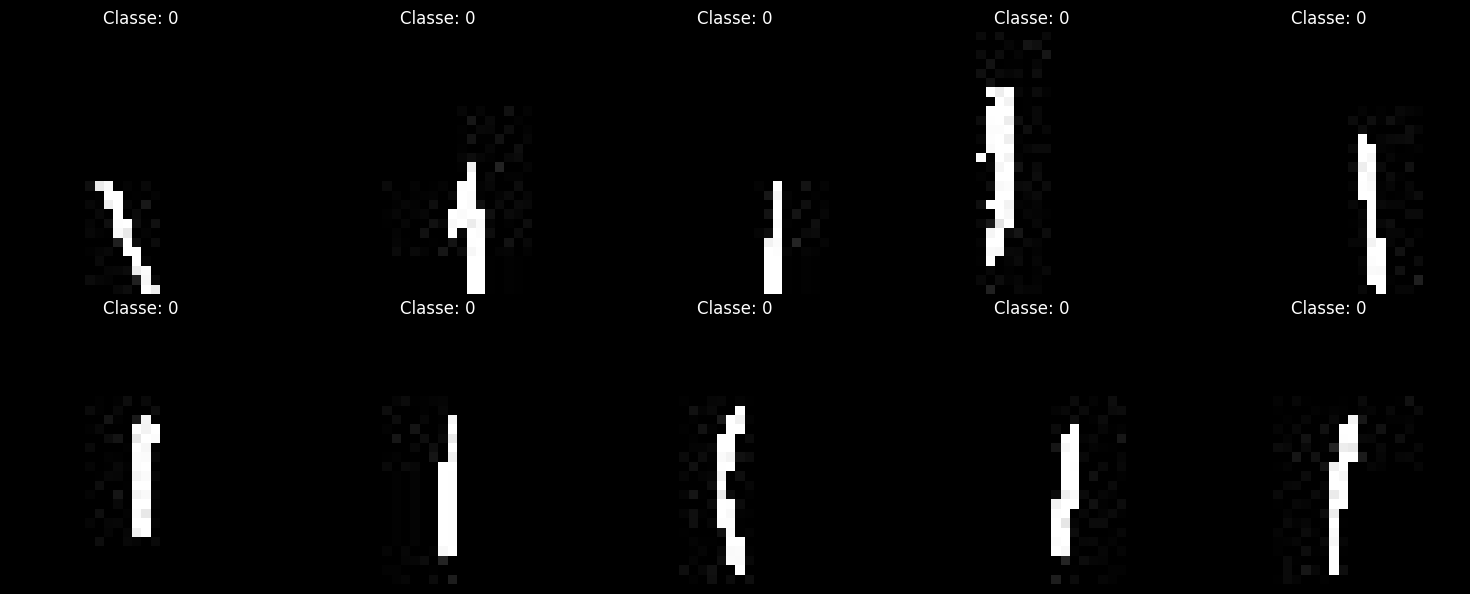
\includegraphics[width=0.7\textwidth]{figures/caractere.png}
\caption{Exemple de caractères ourdous}
\label{fig:urdu_chars}
\end{figure}

Cette visualisation révèle plusieurs caractéristiques importantes :
\begin{itemize}
\item Les caractères apparaissent comme des traits blancs sur fond noir
\item Certains caractères présentent des formes complexes avec des courbes et des angles spécifiques
\item Plusieurs caractères semblent visuellement proches et ne diffèrent que par de petits détails
\item La qualité des images varie, certaines présentant des contours nets tandis que d'autres sont plus bruités
\end{itemize}

\subsection{Distribution des classes}
\begin{flushleft}
L'analyse de la distribution des 40 classes dans le jeu d'entraînement est essentielle pour évaluer l'équilibre du dataset et anticiper d'éventuels biais dans les modèles.
\end{flushleft}

\begin{figure}[H]
\centering
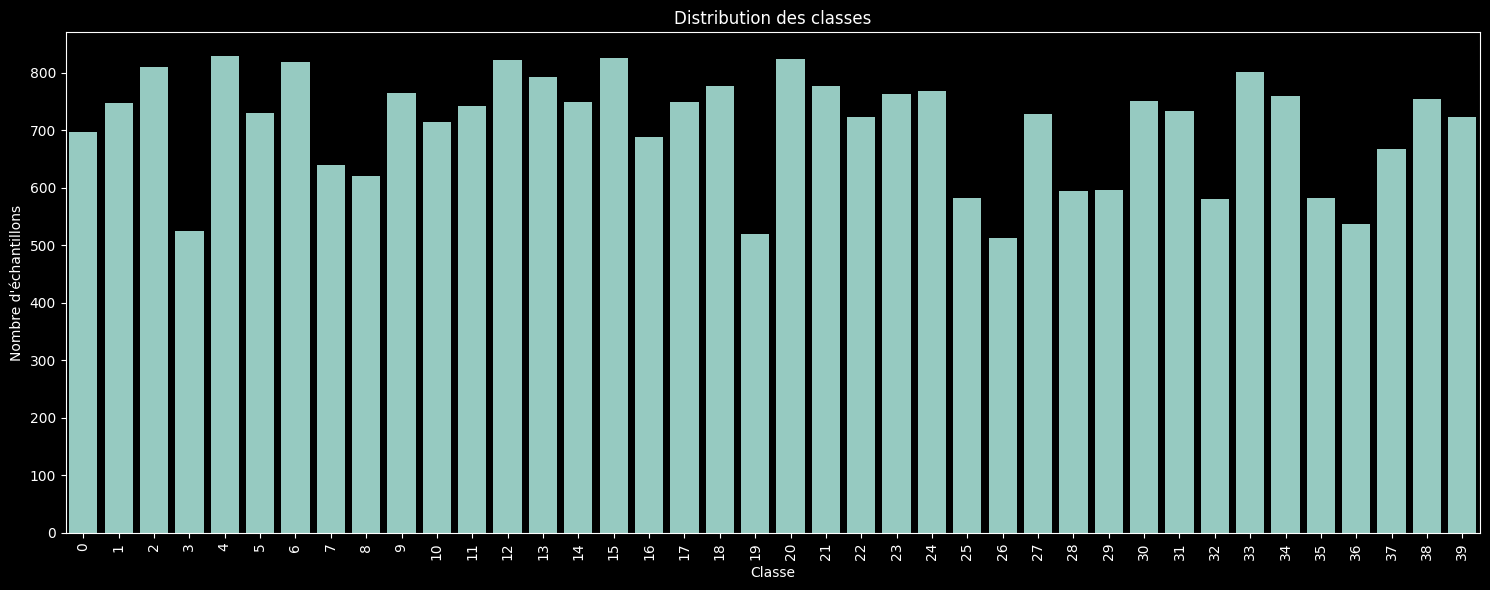
\includegraphics[width=0.7\textwidth]{figures/distribution.png}
\caption{Exemple de caractères ourdous}
\label{fig:urdu_distribution}
\end{figure}

\begin{flushleft}
Comme le montre la figure~\ref{fig:urdu_distribution}, la distribution des classes est relativement équilibrée, avec un nombre d'échantillons par classe variant de 512 (classe 26) à 829 (classe 4). Cette répartition relativement homogène est favorable pour l'entraînement des modèles, minimisant le risque de biais vers les classes surreprésentées.
\end{flushleft}

Les statistiques précises indiquent :


\begin{figure}[h]
\centering
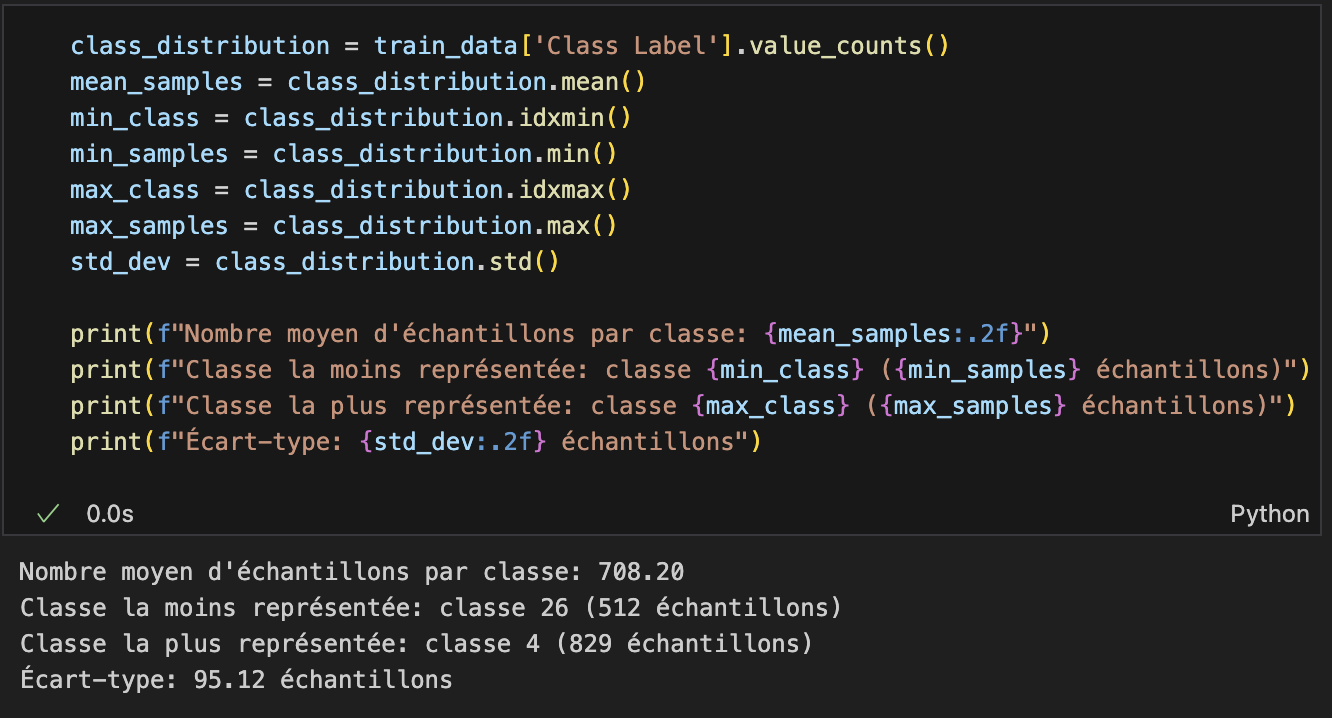
\includegraphics[width=0.7\textwidth]{figures/stat.png}
\caption{les statistiques des classes}
\label{fig:urdu_stat}
\end{figure}

\begin{itemize}
\item Nombre moyen d'échantillons par classe : environ 708
\item Classe la moins représentée : classe 26 (512 échantillons)
\item Classe la plus représentée : classe 4 (829 échantillons)
\item Écart-type : environ 95 échantillons
\end{itemize}

\begin{flushleft}
Cette distribution quasi-équilibrée nous a permis d'utiliser directement les données sans recourir à des techniques de rééchantillonnage, tout en restant vigilants sur la performance des classes moins représentées.
\end{flushleft}

\section{Prétraitement des données}
\begin{flushleft}
Le prétraitement est une étape déterminante pour préparer les données brutes à l'analyse et à la modélisation. Pour ce projet de reconnaissance de caractères ourdou, nous avons appliqué plusieurs transformations essentielles.
\end{flushleft}

\subsection{Normalisation}
\begin{flushleft}
Les valeurs de pixels originales sont comprises entre 0 et 255, ce qui peut créer des gradients importants lors de l'entraînement des modèles de deep learning. Pour faciliter la convergence et améliorer la stabilité de l'apprentissage, nous avons normalisé ces valeurs en les divisant par 255, obtenant ainsi des valeurs dans l'intervalle [0, 1] :
\end{flushleft}

\[
\begin{aligned}
X_{\text{train}} &= \frac{X_{\text{train}}}{255.0} \\
X_{\text{test}} &= \frac{X_{\text{test}}}{255.0}
\end{aligned}
\]

Cette normalisation présente plusieurs avantages :

\begin{itemize}
\item Accélération de la convergence lors de l'entraînement
\item Réduction du risque d'explosion ou de disparition des gradients
\item Standardisation des échelles pour toutes les dimensions d'entrée
\end{itemize}

\subsection{Reshaping pour l'analyse et la modélisation}

Selon l'architecture utilisée, les données ont nécessité différents formats :

\begin{enumerate}
\item \textbf{Pour les MLP :}
\begin{itemize}
\item Format vectoriel aplati (2D) : (n\_samples, 784)
\item Chaque image de 28×28 pixels est transformée en un vecteur de 784 éléments
\end{itemize}
\item \textbf{Pour les CNN :}
\begin{itemize}
\item Format d'image (4D) : (n\_samples, 28, 28, 1)
\item Préservation de la structure spatiale à deux dimensions avec un canal unique (niveaux de gris)
\end{itemize}
\end{enumerate}
\[
\begin{aligned}
X_{\text{train\_cnn}} &= X_{\text{train}}.\text{reshape}(-1,\ 28,\ 28,\ 1) \\
X_{\text{val\_cnn}}   &= X_{\text{val}}.\text{reshape}(-1,\ 28,\ 28,\ 1) \\
X_{\text{test\_cnn}}  &= X_{\text{test}}.\text{reshape}(-1,\ 28,\ 28,\ 1)
\end{aligned}
\]


Cette transformation de format est essentielle pour permettre aux réseaux convolutifs d'exploiter les relations spatiales entre pixels voisins, un aspect fondamental de l'analyse d'images que les MLP ne peuvent pas capturer directement.

\subsection{Division entraînement/validation}

\begin{flushleft}
Pour évaluer rigoureusement la performance des modèles pendant la phase de développement, nous avons divisé l'ensemble d'entraînement en deux sous-ensembles :
\end{flushleft}

\begin{figure}[h]
\centering
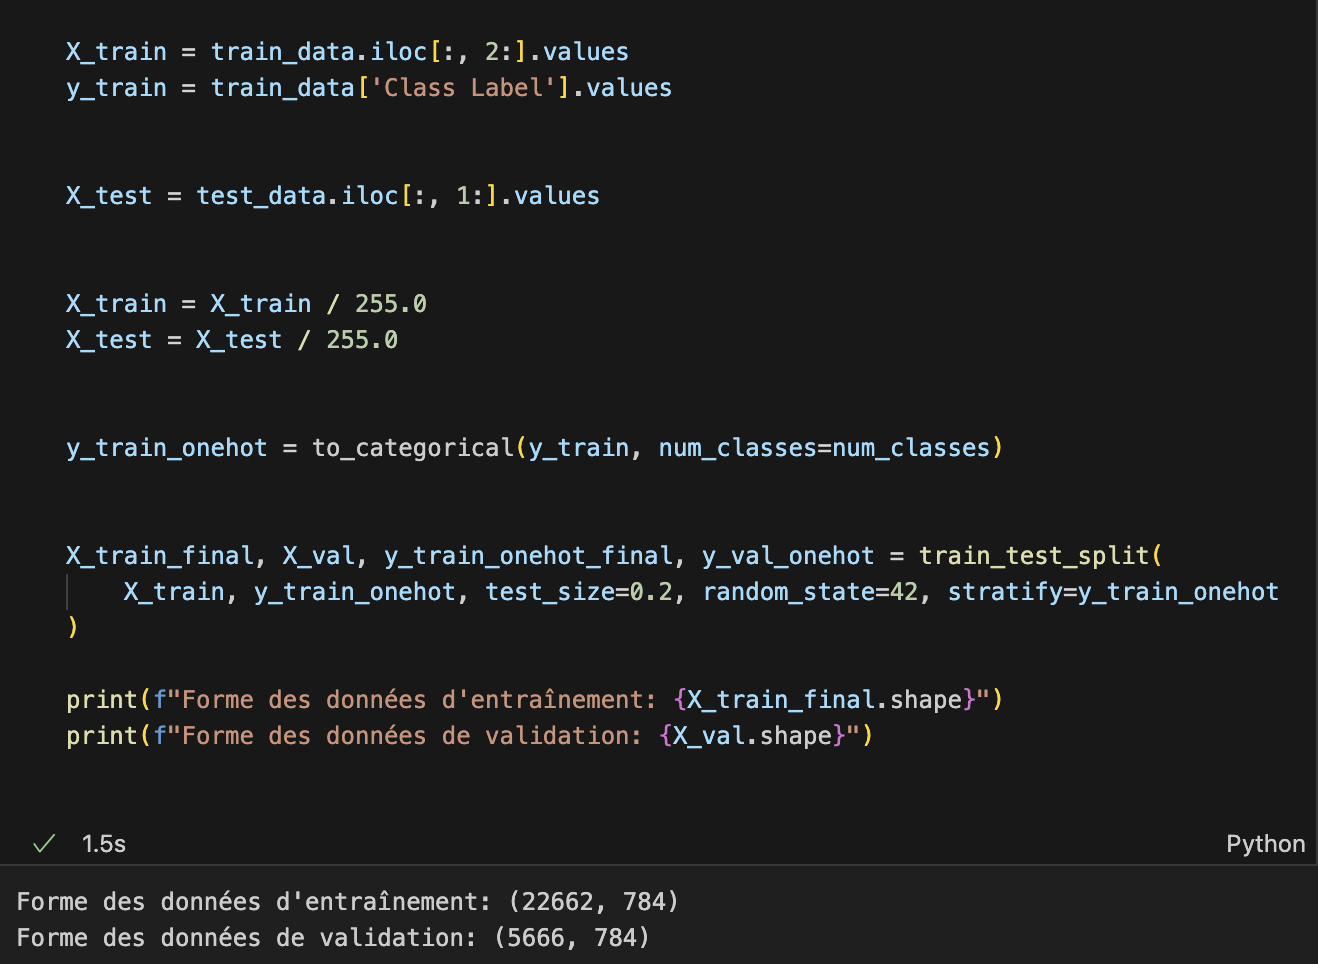
\includegraphics[width=0.7\textwidth]{figures/division.png}
\caption{Division du jeu d'entraînement en entraînement et validation}
\label{fig:urdu_division}
\end{figure}

\begin{itemize}
\item Ensemble d'entraînement final : 80\% des données (= 22 662 échantillons)
\item Ensemble de validation : 20\% des données (= 5 666 échantillons)
\end{itemize}

\begin{flushleft}
La stratification (stratify=y\_train\_onehot) garantit que la distribution des classes dans les ensembles d'entraînement et de validation reste proportionnelle à celle du dataset original, évitant ainsi les biais d'échantillonnage.
\end{flushleft}

\section{Défis spécifiques liés aux caractères ourdou}
\begin{flushleft}
La reconnaissance automatique des caractères ourdou présente plusieurs défis spécifiques qui ont influencé notre approche de modélisation.
\end{flushleft}

\subsection{Complexité morphologique}
\begin{flushleft}
Contrairement aux alphabets latins, les caractères ourdou présentent une morphologie complexe avec des formes curvilignes, des boucles et des traits qui peuvent varier en épaisseur et en orientation. Cette complexité exige des modèles capables de capturer des détails fins et des structures spatiales élaborées.
\end{flushleft}

\subsection{Similarité entre certains caractères}

\begin{flushleft}
Plusieurs caractères ourdou ne diffèrent que par de subtiles variations, comme la position ou le nombre de points diacritiques. Cette similarité peut créer des confusions lors de la classification, comme le révèle l'analyse des matrices de confusion de nos modèles.
\end{flushleft}

\subsection{Variabilité dans la représentation}

\begin{flushleft}
Même au sein d'une même classe, les caractères peuvent présenter des variations stylistiques importantes. Cette variabilité intrinsèque constitue un défi supplémentaire pour les algorithmes d'apprentissage, qui doivent développer une représentation interne suffisamment robuste pour reconnaître un même caractère malgré ces variations.
\end{flushleft}

\subsection{ Qualité et résolution des images}
\begin{flushleft}
La résolution limitée des images (28×28 pixels) peut parfois masquer des détails distinctifs entre caractères similaires. De plus, certaines images présentent des artefacts ou du bruit qui compliquent davantage la tâche de classification.
Ces défis spécifiques ont renforcé notre conviction que des architectures avancées comme les CNN profonds, capables de capturer des caractéristiques hiérarchiques et des relations spatiales complexes, seraient particulièrement adaptées à cette tâche de reconnaissance de caractères ourdou.
\end{flushleft}